\documentclass[14pt, a4paper]{extarticle}

\usepackage[utf8]{inputenc}
\usepackage[russian]{babel}

\usepackage{geometry}
\geometry{
	right=0.39in,
	left=1.18in,
	top=0.3in,
	bottom=0.49in
}

\usepackage{indentfirst}
\setlength\parindent{1.25cm}

%\usepackage{titlesec}
% \titlespacing*{\section}{0pt}{10pt}{0pt}

%\usepackage{titlesec}
%\titleformat{\section}{\normalfont\bfseries}{}{0pt}{}
%\titleformat{\subsection}{\normalfont\itshape}{}{0pt}{}	
	
\usepackage{setspace}
\onehalfspacing

\usepackage{hyperref}

\usepackage[pdftex]{graphicx}
\graphicspath{{png/}}
\DeclareGraphicsExtensions{.pdf,.jpeg,.png}

\usepackage{listings}
\usepackage{xcolor}
\lstset { %
	columns=fullflexible,
	breaklines=true,
	postbreak=\mbox{\textcolor{red}{$\hookrightarrow$}\space},
	backgroundcolor=\color{black!5},
	basicstyle=\footnotesize,
}

\def \deptName {МО ЭВМ}
\def \subjName {Системы реального времени на основе Linux}
\def \labNo {}
\def \labName {Искатель сокровищ}

\def \groupNo {2303}
\def \studName {Канушин М.С.}
\def \proffName {Филатов А.Ю.}

\begin{document}
	
	\begin{titlepage}
	\begin{center}
		\textbf{МИНОБРНАУКИ РОССИИ \\
		САНКТ-ПЕТЕРБУРГСКИЙ ГОСУДАРСТВЕННЫЙ \\	
		ЭЛЕКТРОТЕХНИЧЕСКИЙ УНИВЕРСИТЕТ \\
		<<ЛЭТИ>> ИМ. В.И. УЛЬЯНОВА (ЛЕНИНА) \\
		Кафедра \deptName}
		
		\topskip0pt
		\vspace*{\fill}
			\bigskip\bigskip\bigskip\bigskip\bigskip
			\bigskip\bigskip\bigskip\bigskip\bigskip
			\textbf{ОТЧЕТ \\
			по курсовой работе \labNo \\
			по дисциплине <<\subjName>> \\
			Тема: \labName}
		\vspace*{\fill}
		
		\vspace*{\fill}
		\begin{tabular*}{\textwidth}{l @{\extracolsep{\fill}} r r}
			Студенты гр. \groupNo &  & \studName \\
			 &  & Куришев О.А. \\
			 &  & Черепанов Е.А. \\
			Преподаватель        & \noindent\rule{4cm}{0.4pt} & \proffName \\
		\end{tabular*}
	
		\bigskip\bigskip\bigskip
		\bigskip\bigskip\bigskip
		
		Санкт-Петербург \\
		2018
	\end{center}
	\end{titlepage}

	\setcounter{page}{2}
	\tableofcontents
	\clearpage
	
	\section{Цель работы.}
	\subsection{Постановка задачи}
	Разведать подземелье, найти золото.
	\subsection{Исходные данные}
	Робот ищет золото в подземелье. Робот не знает карту подземелья, должен также определять, в какой части подземелья он находится. Необходимо обойти всё подземелье (также предоставить траекторию перемещения) и найти спрятанные сокровища.
	\subsection{Ограничения на исходные данные}	
	Окружающий мир состоит из прямых линий (комнаты, коридоры). Участки карты, на которых находятся сокровища отличаются от окружающего мира (например, имеют хаотичную, стостящую не из прямых линий, область).
	
	У робота есть лазерный дальномер и данные одометрии.
	
	\section{Обзор используемых пакетов.}
	\textbf{frontier\_exploration}
	Пакет \textit{Frontier Exploration} предоставляет узлы \textit{explore\_client}, \textit{explore\_server}, а также плагин для \textit{coastmap\_2d}.
	
	Предоставленные узлы позволяют запустить задачу исследования территории, заданной пользователем в виде полигона.
	
	\textbf{Navigation Stack}
	Пакет \textit{Navigation Stack} позволяет по данным одометрии и лазерных датчиков передать команды на колеса робота.
	
	\section{Графическое представление системы.}
	На рис. \ref{fig:rqt} представлен rqt graph системы, получившейся при развертывании frontier exploration.
		
	\begin{figure}[h]
		\centering
		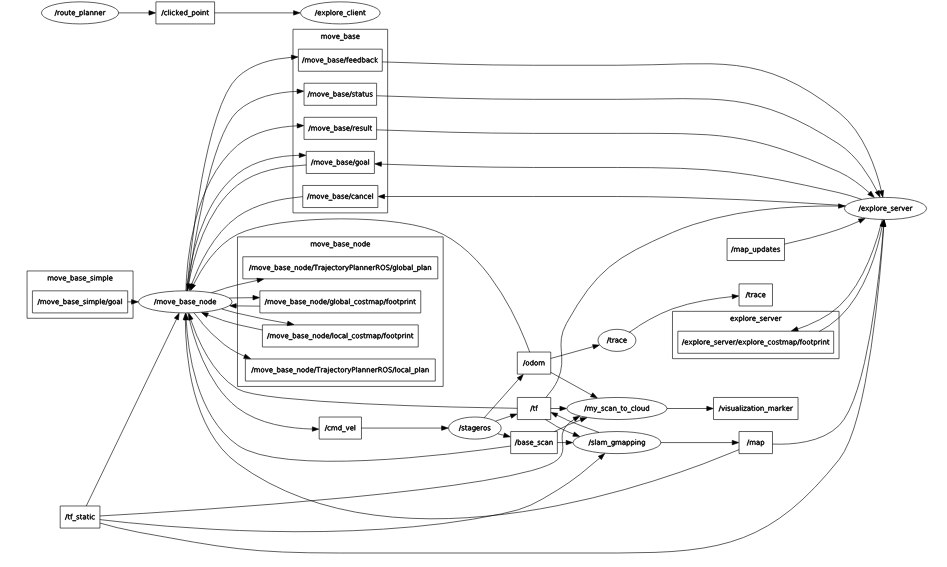
\includegraphics[width=\textwidth]{rqt}
		\caption{Графическое представление системы с помощью Rqt Graph}
		\label{fig:rqt}
	\end{figure}

	Узел Explore server получает данные из tf, move\_base и карты. После анализа полученных данных этот узел генерирует новую цель для робота. Например, при встрече с препятствием, для робота будет сгенерирован новый маршрут, учитывающий расстояние до цели и уже открытую карту.
	
	Ноды route\_planner, trace и my\_scan\_to\_cloud являются вспомогательными. Они были реализованы в данной работе и будут рассмотрены в следующем разделе.
	
	\section{Реализованные узлы.}
	\subsection{trace}
	Данная нода строит маршрут, по которому робот исследовал подземелье. В качестве исходных данных используются данные одометрии, для визуализации в RViz маршрут паблишится как сообщения типа Path в специальный топик.
	
	\subsection{route\_planner}
	Данный узел в автоматическом режиме задает начальную цель для робота. Так как подземелье замкнутое, route planner передает на вход frontier exploration точку, которая находится за пределами этого подземелья. Такой подход позволяет исследовать все подземелье целиком, не пропустив ни одного коридора, так как функционал frontier exploration предусматривает исследование всех возможных путей до тех пор, пока все маршруты не будут изучены.
	
	\subsection{my\_scan\_to\_cloud}
	Поиск сокровищ происходит на основании интенсивности лазерного датчика. При обнаружении сокровища, то есть предмета с заданной интенсивностью, данный узел помечает его и отправляет маркер типа Sphere для визуализации.
	
	\section{Пример работы системы.}
	На рис. \ref{fig:map} представлена карта подземелья (в формате понятном для navigation\_stage), используемая в данном примере для исследования.
	
	\begin{figure}[h]
		\centering
		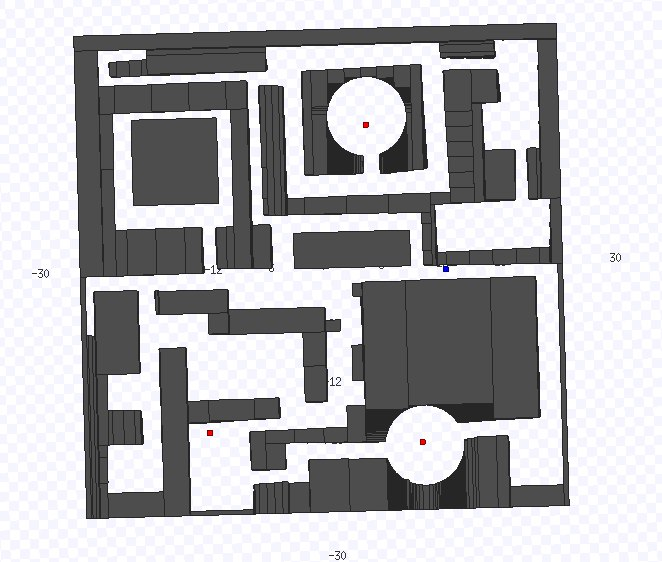
\includegraphics[width=0.7\textwidth]{map}
		\caption{Карта подземелья}
		\label{fig:map}
	\end{figure}

	Синим цветом обозначено местоположение робота, а красным - сокровища, которые необходимо найти.
	
	При обнаружении сокровища, робот отправляет его координаты в виде маркера. На рис. \ref{fig:mesh1} представлено окно RViz в ситуации, когда робот обнаружил первое сокровище.
	
	\begin{figure}[h]
		\centering
		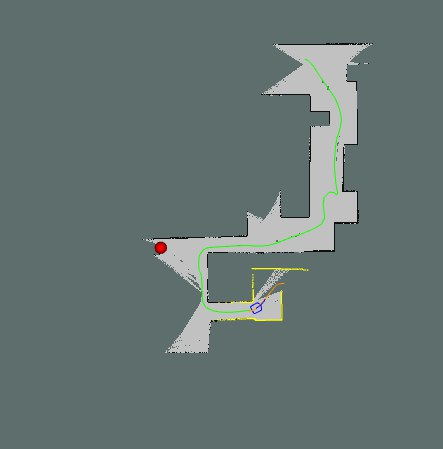
\includegraphics[width=0.7\textwidth]{exp1}
		\caption{Найденное роботом сокровище}
		\label{fig:mesh1}
	\end{figure}

	При обнаружении очередного сокровища отправляется еще один маркер, пример представлен на рис. \ref{fig:mesh2}.

	\begin{figure}[h]
		\centering
		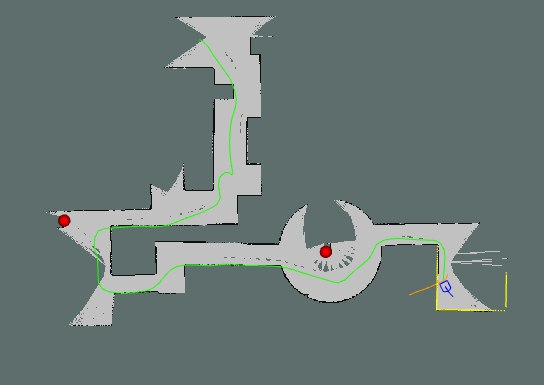
\includegraphics[width=0.7\textwidth]{exp2}
		\caption{Несколько сокровищ, найденных роботом}
		\label{fig:mesh2}
	\end{figure}

	\clearpage
	\section{Код программы.}
	\subsection{scan\_analyzer.cpp}
	\begin{lstlisting}
#include "ros/ros.h"
#include "tf/transform_listener.h"
#include "sensor_msgs/PointCloud.h"
#include "tf/message_filter.h"
#include "message_filters/subscriber.h"
#include "laser_geometry/laser_geometry.h"
#include <visualization_msgs/Marker.h>
#include <nav_msgs/Odometry.h>


class LaserScanToPointCloud{

public:
  int oneMarker;
  ros::Publisher pubMarker;
  ros::Subscriber subOdom;
  nav_msgs::Odometry odmsg;
  visualization_msgs::Marker marker;
  int count;
  ros::NodeHandle n_;
  laser_geometry::LaserProjection projector_;
  tf::TransformListener listener_;
  message_filters::Subscriber<sensor_msgs::LaserScan> laser_sub_;
  tf::MessageFilter<sensor_msgs::LaserScan> laser_notifier_;
  ros::Publisher scan_pub_;

  LaserScanToPointCloud(ros::NodeHandle n) : 
    n_(n),
    laser_sub_(n_, "base_scan", 10),
    laser_notifier_(laser_sub_,listener_, "base_laser_link", 10)
  {
    laser_notifier_.registerCallback(
      boost::bind(&LaserScanToPointCloud::scanCallback, this, _1));
    laser_notifier_.setTolerance(ros::Duration(0.01));
    scan_pub_ = n_.advertise<sensor_msgs::PointCloud>("/my_cloud",1);
    subOdom = n.subscribe("odom", 100,&LaserScanToPointCloud::callback, this);
    pubMarker = n.advertise<visualization_msgs::Marker>("visualization_marker", 10);
   count = 0;
   oneMarker = 0;
  }

void callback(const nav_msgs::Odometry::ConstPtr& msg)
{
   odmsg = *msg;
   std::cout<<"POSE X - "<<odmsg.pose.pose.position.x<<std::endl;
}
void addMarker(float x, float y)
{
        marker.header.frame_id = "base_link";
        marker.header.stamp = ros::Time::now();//ros::Time::now();
        
        // Set the namespace and id for this marker.  This serves to create a unique ID
        // Any marker sent with the same namespace and id will overwrite the old one
        marker.ns = "markersTen";
        marker.id = count;
        count++;
        
        // Set the marker type.  Initially this is CUBE, and cycles between that and SPHERE, ARROW, and CYLINDER
        // marker.type = shape;
        marker.type = visualization_msgs::Marker::SPHERE;
        marker.action = visualization_msgs::Marker::ADD;
        
        // Set the pose of the marker.  This is a full 6DOF pose relative to the frame/time specified in the header
      
        marker.pose.position.x = x;//odmsg.pose.pose.position.x;
        marker.pose.position.y = y;//odmsg.pose.pose.position.y;

        marker.pose.position.z = 0;
        marker.pose.orientation.x = 0.0;
        marker.pose.orientation.y = 0.0;
        marker.pose.orientation.z = 0.0;
        marker.pose.orientation.w = 1.0;
        
        // Set the scale of the marker -- 1x1x1 here means 1m on a side
        marker.scale.x = 1.0;
        marker.scale.y = 1.0;
        marker.scale.z = 1.0;
        
        // Set the color -- be sure to set alpha to something non-zero!
        marker.color.r = 1.0f;
        marker.color.g = 0.0f;
        marker.color.b = 0.0f;
        marker.color.a = 1.0;

        marker.lifetime = ros::Duration();
       
	
	pubMarker.publish(marker);

      
}

  void scanCallback (const sensor_msgs::LaserScan::ConstPtr& scan_in)
  {
    int count = 0;

    sensor_msgs::PointCloud cloud;
    try
    {
        projector_.transformLaserScanToPointCloud(
          "base_laser_link",*scan_in, cloud,listener_);
    }
    catch (tf::TransformException& e)
    {
        std::cout << e.what();
        return;
    }

    int i = 0;
    float x;
    float y;
    for(  i = 0; i < 100; i++)
    {
       if (scan_in->intensities[i] == 2) 
       {
	std::cout<<"I see the treasure"<<std::endl;
        x = cloud.points[i].x;
        y = cloud.points[i].y;
	oneMarker = 1;
	break;
       }
    } 
    if (oneMarker == 1)
    {
	addMarker(x,y);
	oneMarker = 0;
        ros::Duration(10).sleep();
    } 
  }
};

int main(int argc, char** argv)
{
  
  ros::init(argc, argv, "my_scan_to_cloud");
  ros::NodeHandle n;
  LaserScanToPointCloud lstopc(n);
  
  ros::spin();
  
  return 0;
}
\end{lstlisting}

	\subsection{trace.py}
\begin{lstlisting}
#!/usr/bin/env python

from geometry_msgs.msg import PoseStamped
from nav_msgs.msg import Path, Odometry
from rospy import Duration, Publisher as Pub, Subscriber as Sub, Timer
from rospy import init_node, spin


class LocationFinder:
    def __init__(self):
        self.position = None
        Sub('/odom', Odometry, self._callback)

    def _callback(self, odometry):
        self.position = odometry.pose.pose.position


class Trace:
    def __init__(self):
        self.pub = Pub('/trace', Path, queue_size=100)
        self.loc = LocationFinder()
        self.path = Path()
        self.path.header.frame_id = 'odom'
        Timer(Duration.from_sec(1), self._path)

    def _path(self, _):
        p = PoseStamped()
        p.header.frame_id = 'odom'
        p.pose.position = self.loc.position
        self.path.poses.append(p)

        self.pub.publish(self.path)


if __name__ == '__main__':
    init_node(Trace.__name__)

    Trace()

    spin()
\end{lstlisting}

	\subsection{route\_planner.py}
\begin{lstlisting}
#!/usr/bin/env python

from geometry_msgs.msg import PointStamped as Point
from rospy import Publisher as Pub
from rospy import sleep, spin, init_node


class RoutePlanner:
    def __init__(self):
        self.pub = Pub('/clicked_point', Point, queue_size=100)

    def _publish_point(self, x, y):
        sleep(0.5)
        p = Point()
        p.header.frame_id = 'map'
        p.point.x = float(x)
        p.point.y = float(y)
        self.pub.publish(p)

    def go(self, x, y):
        self._publish_point(x - 1, y - 1)
        self._publish_point(x + 1, y - 1)
        self._publish_point(x, y + 1)
        self._publish_point(x - 1, y - 1)

        self._publish_point(x, y)

    def explore(self):
        self._publish_point(-100, -100)
        self._publish_point(-100, 100)
        self._publish_point(100, 100)
        self._publish_point(100, -100)
        self._publish_point(-100, -100)
        self._publish_point(0, 0)


if __name__ == '__main__':
    init_node(RoutePlanner.__name__)

    target = RoutePlanner()
    target.go(16, -21)

    spin()
\end{lstlisting}

	\subsection{treasure\_hunter.launch}
\begin{lstlisting}
<launch>
  <node name="trace" pkg="treasure_hunter" type="trace.py" respawn="true"/>
  <node name="route_planner" pkg="treasure_hunter" type="route_planner.py" respawn="true"/>
  <node name="my_scan_to_cloud" pkg="treasure_hunter" type="scan_analyzer" respawn="true"/>
</launch>
\end{lstlisting}

\end{document}